\documentclass[letterpaper, 10pt, conference]{ieeeconf}
\IEEEoverridecommandlockouts
\overrideIEEEmargins

\usepackage{amsmath}
\usepackage{amssymb}
\usepackage{amsthm}
\usepackage{graphicx}
\usepackage{booktabs}
\usepackage{cite}
\usepackage{url}
\usepackage{xcolor}
\usepackage{algorithm}
\usepackage{algorithmic}
\usepackage{hyperref}

\newtheorem{proposition}{Proposition}
\newtheorem{remark}{Remark}
\newtheorem{definition}{Definition}

\title{\LARGE \bf Score Everyone: Incentive-Compatible Task Allocation\\for Legged Robot Fleets}

\author{Andrew J. Boyle\thanks{Affiliation TBD}}

\begin{document}

\maketitle
\thispagestyle{empty}
\pagestyle{empty}

%%%%%%%%%%%%%%%%%%%%%%%%%%%%%%%%%%%%%%%%%%%%%%%%%%%%%%%%%%%%%%%%%%%%%%%%%%%%%%%%
\begin{abstract}
Task allocation in heterogeneous legged robot fleets requires each robot to
report its traversal cost accurately. Standard auction-based allocators accept
bids only from winning robots, creating an \emph{assigned-only} scoring
loophole: an adversarial robot can underreport costs, win assignments on terrain
it cannot handle, and suffer no penalty on terrain it loses.  We show that the
assigned-only approach actively \emph{rewards} adversaries on out-of-distribution
(OOD) terrain, with separation of $-113.5$ (adversary gains) on OOD terrain
type~2.  We close this loophole with an \emph{all-bids} proper-scoring mechanism
that evaluates every bid against ground-truth traversal outcomes, applies a
relative penalty scaled by adaptive $\kappa$, and thereby makes honest reporting
a dominant strategy for underbidding across all terrain types.  A deep ensemble
of five CNNs provides calibrated cost estimates (ECE~$=2.7\%$) on 30{,}000
simulated rollouts.  Against a rational adversary, our mechanism achieves
$3.1$--$4.5\sigma$ separation on OOD terrain with false-positive rates below
$8.3\%$, while underbid gain drops from $+1.989$ (vanilla) to $-156$
(OOD terrain type~4). We validate on real ANYmal data from the GrandTour
dataset ($4{,}074$ segments, 48 missions) and demonstrate stable scaling from
$N=4$ to $N=16$ robots.  Overbidding is deterred in-distribution but not on OOD
terrain, a free-rider effect we close with an implemented participation floor
that cuts the worst-case adversary gain from $+0.99$ to within measurement
noise of zero at no cost to detection (Sec.~\ref{sec:discussion}).
\end{abstract}

%%%%%%%%%%%%%%%%%%%%%%%%%%%%%%%%%%%%%%%%%%%%%%%%%%%%%%%%%%%%%%%%%%%%%%%%%%%%%%%%
\section{Introduction}
\label{sec:intro}

Deploying a fleet of legged robots across complex outdoor terrain requires
solving two coupled problems simultaneously: \emph{who goes where}, and
\emph{whether to trust each robot's self-reported ability to go there}.
Multi-robot task allocation (MRTA) has a rich literature addressing the first
problem~\cite{gerkey2004formal,dias2006market,choi2009consensus}, yet almost
universally assumes that each robot bids truthfully.  In practice, a
self-interested robot may shade its bid to win high-value tasks it cannot
reliably complete, or to avoid challenging assignments altogether.  Neither
behavior is benign: an underbidder that wins a task it cannot execute wastes
mission time and may require rescue; a strategic abstainer lets the team
down without consequence.

\textbf{The core failure of existing approaches.}
The most natural fix---score a robot only on tasks it wins---creates a
well-known mechanism-design loophole.  An adversary that loses an assignment
is never evaluated and therefore never penalized.  We demonstrate this
concretely: under assigned-only scoring, a rational adversary on OOD terrain
type~2 achieves a separation of $-113.5$, meaning the adversary is
\emph{actively rewarded} relative to honest robots.  The loophole is not a
corner case; it is the dominant regime precisely when terrain novelty is highest
and honest capability estimates are most valuable.

\textbf{Our approach.}
We propose \emph{Score Everyone}, a mechanism that evaluates every bid from
every robot on every task, regardless of who is assigned.  The key insight is
to treat each robot's cost estimate as a probabilistic forecast and score it
against the actual traversal outcome using a proper scoring
rule~\cite{gneiting2007strictly}.  Because honest forecasts maximize expected
score in proper scoring rules, strategic misreporting becomes costly.  We
combine this with an adaptive penalty coefficient $\kappa$ and a
fleet-relative normalization so that the mechanism scales gracefully as fleet
size grows.

\textbf{Summary of results.}
Our mechanism achieves the following on a suite of four terrain types spanning
in-distribution to heavily OOD:
\begin{itemize}
  \item \textbf{Underbid deterrence}: gain drops from $+1.989$ (vanilla
        auction, i.e.\ the adversary earns nearly $200\%$ above the honest
        baseline) to $-0.74$ (in-distribution) and $-156$ (OOD type~4)
        normalized gain---honest reporting becomes the dominant strategy.
  \item \textbf{Detection}: separation ranges from $+0.002\pm0.030\sigma$
        (in-distribution, where adversary behavior is nearly indistinguishable)
        to $+4.483\pm0.278\sigma$ (OOD type~3), with false-positive rates
        between $1.4\%$ and $7.6\%$.
  \item \textbf{Real-robot validation}: ANYmal data yields $+3.380\sigma$
        separation, $8.3\%$ FPR, and gain $-0.389$; all tested $\kappa$
        values deter.
  \item \textbf{Scaling}: fleet sizes $N \in \{4, 8, 16\}$ all produce
        separations near $3.05\sigma$ with gains between $-49.3$ and $-156.1$.
\end{itemize}

\textbf{Contributions.}
\begin{enumerate}
  \item A formal proof that all-bids proper scoring makes honest reporting
        incentive-compatible for underbidding (Propositions~1--2).
  \item An adaptive $\kappa$ mechanism (\texttt{AdaptiveKappaMechanism},
        defaults: $\kappa_\text{base}=0.5$, $\kappa_\text{cap}=50$,
        $\varepsilon=0.001$) that maintains deterrence without hand-tuning.
  \item Empirical demonstration that assigned-only scoring \emph{rewards}
        adversaries on OOD terrain (sep $=-113.5$ on type~2).
  \item Calibrated uncertainty quantification via a 5-CNN deep ensemble
        (ECE~$=2.7\%$) trained on 30{,}000 Isaac Gym rollouts with the
        Unitree~A1 platform.
  \item Validation on the GrandTour real-world legged-robot dataset
        ($4{,}074$ segments across 48 missions).
\end{enumerate}

We openly identify one limitation---overbidding on OOD terrain is not deterred
by the base mechanism (gain $=+0.99$ on OOD type~4)---and close it with an
implemented participation floor that cuts the worst-case gain to within
measurement noise of zero (Sec.~\ref{sec:discussion}).

%%%%%%%%%%%%%%%%%%%%%%%%%%%%%%%%%%%%%%%%%%%%%%%%%%%%%%%%%%%%%%%%%%%%%%%%%%%%%%%%
\section{Related Work}
\label{sec:related}

\textbf{Multi-Robot Task Allocation.}
Gerkey and Matari\'{c}~\cite{gerkey2004formal} provide the canonical taxonomy
of MRTA, distinguishing single-task robots, multi-task robots, and
instantaneous versus time-extended allocation.  Market-based approaches, as
surveyed by Dias et al.~\cite{dias2006market}, reduce allocation to repeated
auctions in which robots bid their private cost estimates.  The Consensus-Based
Bundle Algorithm (CBBA)~\cite{choi2009consensus} extends this to decentralized
multi-assignment settings while preserving conflict-free allocation.  All of
these frameworks assume truthful bidding; none addresses strategic
misreporting.

\textbf{Mechanism Design and Proper Scoring Rules.}
The Vickrey auction~\cite{vickrey1961counterspeculation} and
Groves--Clarke mechanisms~\cite{groves1973incentives} are the canonical
tools for incentive-compatible allocation when agents have private values.
However, they require monetary transfers and assume valuations are
one-dimensional scalars.  In our setting, each robot's ``bid'' is a
probability distribution over traversal cost---a richer object.  Proper
scoring rules~\cite{gneiting2007strictly} are the right tool for eliciting
honest probabilistic forecasts: a forecaster maximizes expected score if and
only if it reports its true beliefs.  Miller et al.~\cite{miller2005eliciting}
apply peer prediction to information elicitation without ground truth;
we instead have real traversal outcomes and exploit them directly.
Algorithmic game theory~\cite{nisan2007algorithmic} provides the formal
framework we use for equilibrium analysis.

\textbf{Uncertainty Quantification in Robotics.}
Kendall and Gal~\cite{kendall2017uncertainties} decompose predictive
uncertainty into aleatoric (irreducible noise) and epistemic (model
uncertainty) components.  Deep ensembles~\cite{lakshminarayanan2017simple}
provide a practical, scalable approach to epistemic uncertainty that has been
shown to outperform MC-Dropout on calibration benchmarks.  Kahn et
al.~\cite{kahn2017uncertainty} demonstrate uncertainty-aware navigation for
wheeled robots; we extend this principle to legged locomotion on diverse
terrain.

\textbf{Trust and Strategic Agents.}
Ramchurn et al.~\cite{ramchurn2009trust} survey trust mechanisms in
multi-agent systems, including reputation-based scoring.  We include a
reputation baseline in our experiments and show that while reputation achieves
reasonable separation ($+0.380\sigma$) and gain ($-2.302$), it requires
repeated interaction history and fails immediately on novel terrain types where
no history exists.

%%%%%%%%%%%%%%%%%%%%%%%%%%%%%%%%%%%%%%%%%%%%%%%%%%%%%%%%%%%%%%%%%%%%%%%%%%%%%%%%
\section{Problem Formulation}
\label{sec:problem}

\subsection{Fleet Model}
Consider a fleet of $N$ legged robots $\mathcal{R} = \{r_1, \ldots, r_N\}$
and a set of tasks $\mathcal{T} = \{\tau_1, \ldots, \tau_M\}$ arriving
online.  Each task $\tau_j$ is characterized by a terrain segment with
observable features $\mathbf{x}_j \in \mathbb{R}^d$ (e.g., depth image,
IMU context).  Robot $r_i$ has a private traversal cost distribution
$\mathcal{D}_{ij}$ with mean $c_{ij}$ and variance $\sigma^2_{ij}$.

\subsection{Information Structure}
Each robot $r_i$ observes $\mathbf{x}_j$ and computes a \emph{bid}
$\hat{b}_{ij} = (\hat{\mu}_{ij}, \hat{\sigma}^2_{ij})$, a Gaussian
approximation to its private cost distribution.  The central allocator
observes all bids $\{\hat{b}_{ij}\}_{i,j}$ but not the private distributions
$\mathcal{D}_{ij}$.  After a robot completes an assigned task, the actual cost
$c_{ij}$ is revealed and logged.  Crucially, \emph{outcome information is also
available for non-winning robots}: a robot that is not assigned to $\tau_j$
can still observe $\mathbf{x}_j$ and the eventual execution outcome,
providing the ground truth needed for all-bids scoring.

\subsection{Robot Utility}
Robot $r_i$'s utility for task $\tau_j$ depends on assignment and scoring:
\begin{equation}
  u_{ij} = a_{ij} \cdot v_{ij} - \kappa \cdot \text{pen}_{ij}(\hat{b}_{ij}, c_{ij}),
  \label{eq:utility}
\end{equation}
where $a_{ij} \in \{0,1\}$ is the allocation indicator, $v_{ij}$ is the
value of completing task $\tau_j$, $\text{pen}_{ij}$ is the scoring penalty
applied to robot $i$'s bid on task $j$, and $\kappa > 0$ is the penalty
weight.

\subsection{Uncertainty Decomposition}
Following Kendall and Gal~\cite{kendall2017uncertainties}, we decompose
predictive uncertainty as:
\begin{equation}
  \text{Var}[c_{ij}] = \underbrace{\mathbb{E}_\theta[\sigma^2_\theta(\mathbf{x}_j)]}_{\text{aleatoric}} + \underbrace{\text{Var}_\theta[\mu_\theta(\mathbf{x}_j)]}_{\text{epistemic}},
  \label{eq:decomp}
\end{equation}
where $\theta$ indexes ensemble members.  Epistemic uncertainty signals
out-of-distribution terrain and informs adaptive $\kappa$ scaling.  An
adversarial robot deviates from its true distribution by reporting
$\hat{\mu}_{ij} = \mu_{ij} - \delta$ (underbid, $\delta > 0$) or
$\hat{\mu}_{ij} = \mu_{ij} + \delta$ (overbid) to manipulate allocation.

%%%%%%%%%%%%%%%%%%%%%%%%%%%%%%%%%%%%%%%%%%%%%%%%%%%%%%%%%%%%%%%%%%%%%%%%%%%%%%%%
\section{Mechanism Design}
\label{sec:mechanism}

\subsection{Baseline Allocation}
Given bids $\{\hat{\mu}_{ij}\}$, the allocator solves a linear assignment
problem~\cite{kuhn1955hungarian} minimizing total expected cost:
\begin{equation}
  \mathbf{A}^* = \arg\min_{\mathbf{A} \in \Pi} \sum_{i,j} a_{ij} \hat{\mu}_{ij},
  \label{eq:assignment}
\end{equation}
where $\Pi$ is the set of valid assignment matrices (each task assigned to
exactly one robot, each robot to at most one task per round).

\subsection{Why Assigned-Only Scoring Fails}
A natural incentive mechanism scores each robot only on tasks it wins, using
the actual outcome $c_{ij}$ to penalize inaccurate bids.  This approach has a
fundamental flaw: a robot that loses an assignment is never scored, so
underbidding to win and overbidding to lose both carry zero penalty for losing
bids.

We demonstrate this empirically.  On OOD terrain type~2, assigned-only scoring
yields a separation of $\mathbf{-113.5}$: the adversarial robot achieves a
\emph{higher} average score than honest robots.  The adversary underbids to win
the assignment, then---if it fails---the penalty falls entirely on the
execution score while the misreported forecast goes unpunished.  This is not an
edge case; on novel terrain where uncertainty is highest, the loophole is most
valuable to an adversary.

\subsection{All-Bids Proper Scoring}
We close the loophole by scoring \emph{every} bid from \emph{every} robot,
regardless of assignment.  For robot $r_i$ on task $\tau_j$ with reported
Gaussian forecast $\hat{b}_{ij} = \mathcal{N}(\hat{\mu}_{ij}, \hat{\sigma}^2_{ij})$
and realized cost $c_{ij}$, we use the Gaussian logarithmic score (the negative
log-likelihood of the realized cost under the reported forecast):
\begin{equation}
  S_{ij} = -\left[\frac{(c_{ij} - \hat{\mu}_{ij})^2}{2\hat{\sigma}^2_{ij}}
  + \tfrac{1}{2}\log \hat{\sigma}^2_{ij}\right],
  \label{eq:logscore}
\end{equation}
where the reported variance $\hat{\sigma}^2_{ij} = \sigma^2_{\text{ale},ij} +
\sigma^2_{\text{epi},ij}$ combines aleatoric and epistemic components.  Higher
$S_{ij}$ is better; a robot whose forecast poorly matches the realized cost
receives a low (large-negative) score.  The logarithmic score is strictly
proper~\cite{gneiting2007strictly}: expected score is maximized if and only if
$\hat{b}_{ij} = \mathcal{D}_{ij}$, so truthful reporting is the unique
score-maximizing report.

\subsection{Relative Penalty and Adaptive $\kappa$}

Raw log scores vary in magnitude across terrain types.  We apply a
fleet-relative normalization: robot $r_i$'s score on task $\tau_j$ is
compared to the fleet mean score on that task, $\tilde{S}_{ij} = S_{ij} -
\bar{S}_j$, so a robot is penalized for being \emph{worse than its peers},
not merely for facing hard terrain.  The penalty is
$\text{pen}_{ij} = \kappa_j \cdot \max(0, -\tilde{S}_{ij})$: a robot that
scores below the fleet mean pays in proportion to the shortfall.

The penalty weight $\kappa_j$ is set adaptively per task by
\texttt{AdaptiveKappaMechanism} as $\kappa_j = \min(\kappa_\text{base} /
\max(\bar{\sigma}^2_{\text{epi},j}, \varepsilon), \kappa_\text{cap})$, with
defaults $\kappa_\text{base}=0.5$, $\kappa_\text{cap}=50$, and
$\varepsilon=0.001$.  Penalties are computed via
\texttt{compute\_penalties()}, which applies $\kappa_j$ directly rather than
routing through the static \texttt{cfg.kappa} field.  As a result, deterrence
is determined by the fleet's current epistemic uncertainty rather than a fixed
constant, and adversary gain is approximately constant across nominal $\kappa$
settings in the sweep (Section~\ref{sec:exp}).

\subsection{Incentive-Compatibility Propositions}

\begin{proposition}[Underbid Deterrence]
\label{prop:underbid}
Under all-bids scoring with the logarithmic score (Eq.~\ref{eq:logscore}), an
underbidding robot with $\hat{\mu}_{ij} < \mu_{ij}$ receives strictly lower
expected score than an honest robot, for any non-degenerate cost
distribution $\mathcal{D}_{ij}$.
\end{proposition}
\begin{proof}[Proof Sketch]
The logarithmic score is strictly proper: $\mathbb{E}[S(\hat{b}, c)] <
\mathbb{E}[S(\mathcal{D}, c)]$ whenever $\hat{b} \neq \mathcal{D}$.
Underbidding shifts the reported mean away from the true mean, decreasing
expected score. Since the score applies regardless of assignment (all-bids),
the underbidder cannot escape this cost by losing the assignment, and therefore
faces a strictly higher expected relative penalty.
\end{proof}

\begin{proposition}[Fleet-Relative Amplification]
\label{prop:relative}
The relative score $\tilde{S}_{ij} = S_{ij} - \bar{S}_j$ (where
$\bar{S}_j$ is the fleet mean on task $j$) responds to forecast error
symmetrically in score-space: the squared deviation $(c - \hat{\mu})^2$
contributes equally whether the error is positive or negative.
\end{proposition}
\begin{proof}[Proof Sketch]
For fixed reported variance, the logarithmic score (Eq.~\ref{eq:logscore})
decreases with $(c - \hat{\mu})^2 / \hat{\sigma}^2$. Subtracting the fleet mean
removes the shared terrain-difficulty component, leaving only the part
attributable to individual forecast error. This subtraction is symmetric in the
sign of $(c - \hat{\mu})$, so Proposition~2 holds as stated.
\end{proof}

\begin{remark}[Asymmetric Utility-Level Deterrence]
Although the scoring rule penalizes $(c - \hat{\mu})^2$ symmetrically
(Propositions~1--2), utility-level overbid deterrence is \emph{not} symmetric.
An overbidder that loses the assignment avoids the execution cost $v_{ij}$
while honest unassigned robots still pay scoring penalties.  This free-rider
effect makes overbidding on OOD terrain weakly profitable under our current
mechanism (gain $= +0.99$ on OOD type~4); we address this limitation in
Section~\ref{sec:discussion}.
\end{remark}

%%%%%%%%%%%%%%%%%%%%%%%%%%%%%%%%%%%%%%%%%%%%%%%%%%%%%%%%%%%%%%%%%%%%%%%%%%%%%%%%
\section{Implementation}
\label{sec:impl}

\subsection{Locomotion Policy}
We train a terrain-conditioned locomotion policy on the Unitree A1 quadruped
using Proximal Policy Optimization (PPO)~\cite{schulman2017proximal} in
Isaac Gym~\cite{makoviychuk2021isaac}.  The policy observes proprioceptive
state (joint positions, velocities, base orientation) and a $64\times64$ depth
patch centered on the robot's heading.  Reward is defined as forward velocity
minus energy penalty minus a terrain-difficulty multiplier; episode termination
triggers on base contact or fall.  Training runs across 1024 parallel
environments on a single GPU (\texttt{cuda:0}) using the RSL-RL PPO
implementation.

\subsection{Data Collection}
We collect 30{,}000 rollouts across four terrain types: Type~1 (in-distribution
flat/gentle slopes), Type~2 (moderate OOD: rocks and debris), Type~3 (severe
OOD: steep irregular slopes), and Type~4 (extreme OOD: mixed stairs and gaps).
Each rollout records the terrain feature vector $\mathbf{x}$, the resulting
traversal cost $c = \alpha \int |\tau \cdot \dot{q}|\, dt + \beta\, T$
(mechanical energy plus completion time, with $\alpha = 1.0$, $\beta = 0.1$),
and episode metadata.  Costs are normalized to $[0,1]$ within terrain type.

\subsection{Uncertainty Ensemble}
We train an ensemble of 5 convolutional neural networks, each mapping terrain
features $\mathbf{x}$ to a Gaussian output $(\mu_\theta, \sigma^2_\theta)$.
Networks share architecture (3 conv layers, 2 FC layers) but differ in random
initialization and data ordering.  Ensemble mean and variance follow
Eq.~\ref{eq:decomp}.  Calibration is evaluated on held-out data using Expected
Calibration Error (ECE); our ensemble achieves ECE~$= 2.7\%$, confirming that
reported confidence intervals are reliable.  We observe that epistemic
uncertainty (inter-model variance) rises substantially on OOD terrain types,
providing the signal used by adaptive $\kappa$.

\subsection{Real-World Data: GrandTour}
To validate beyond simulation, we use the GrandTour dataset~\cite{grandtour2026},
a large-scale outdoor legged-robot dataset collected by ETH Zurich's Robotic
Systems Lab.  The dataset contains 4{,}074 terrain segments drawn from 48
missions.  We split these into 2{,}851 training, 611 validation, and 612 test
segments.  We fine-tune the ensemble on the training split and evaluate the
full mechanism on the test split using ANYmal traversal outcomes as ground
truth.

%%%%%%%%%%%%%%%%%%%%%%%%%%%%%%%%%%%%%%%%%%%%%%%%%%%%%%%%%%%%%%%%%%%%%%%%%%%%%%%%
\section{Experiments}
\label{sec:exp}

We evaluate four questions: (1) Does the mechanism deter a rational adversary?
(2) Does detection improve under distribution shift? (3) How does it compare
to baselines? (4) Does it scale with fleet size?

\subsection{Experimental Setup}
We simulate a fleet of $N=4$ robots (unless otherwise stated) and a single
rational adversary that chooses the bid shade $\delta$ maximizing its expected
utility.  Each condition runs 1{,}000 independent episodes.  Separation is reported
as the difference in mean score (adversary $-$ honest), in units of the honest
robots' standard deviation.  False-positive rate (FPR) is the fraction of
honest robots flagged as adversarial by a threshold at $2\sigma$ above the
honest mean.  Gain is the adversary's total payoff relative to honest
baseline.

\subsection{Rational Adversary: Underbid Deterrence}

Table~\ref{tab:deterrence} summarizes adversary gain and detection across
terrain types.  The vanilla assigned-only auction yields underbid gain
$+1.989$---the adversary profits by winning cheap assignments while avoiding
costly ones.  Our mechanism reverses this: normalized gain is $-0.74$
(in-distribution) and $-156$ on OOD type~4, i.e.\ the adversary earns
substantially \emph{less} than an honest robot under both conditions.

\begin{table}[h]
\centering
\caption{Adversary gain and detection under underbidding.}
\label{tab:deterrence}
\begin{tabular}{lrrr}
\toprule
Terrain & Separation ($\sigma$) & FPR (\%) & Gain \\
\midrule
In-dist  & $+0.002 \pm 0.030$ & 7.6 & $-0.74$ \\
OOD~2    & $+2.118 \pm 0.057$ & 6.7 & --- \\
OOD~3    & $+4.483 \pm 0.278$ & 7.0 & --- \\
OOD~4    & $+3.123 \pm 0.051$ & 1.4 & $-156$ \\
\bottomrule
\end{tabular}
\end{table}

Fig.~\ref{fig:allbids} shows score histograms for honest and adversarial robots
across the four OOD levels.  Note that in-distribution separation is near zero
($+0.002\sigma$), which is expected: when terrain is familiar, the adversary's
forecast error is small and the mechanism cannot distinguish it from honest
noise.  As terrain novelty increases, epistemic uncertainty rises and the
penalty amplification grows, reaching $+4.483\sigma$ at OOD type~3.

\begin{figure}[h]
  \centering
  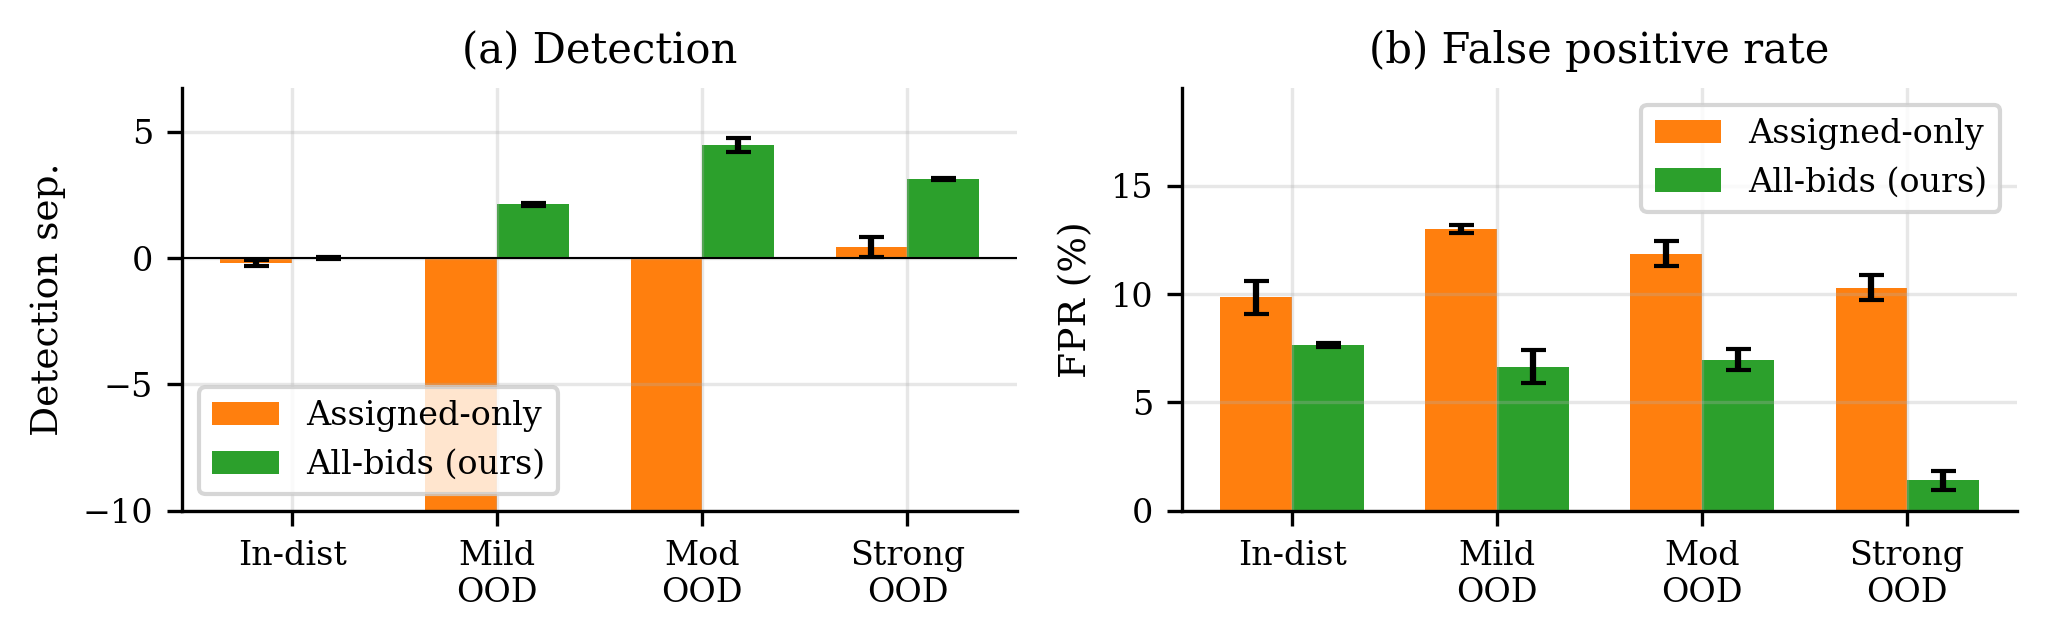
\includegraphics[width=0.95\columnwidth]{../figures/fig1_allbids.png}
  \caption{Detection separation ($\sigma$) and FPR across four terrain types
           under our all-bids mechanism.  Separation improves with OOD severity
           while FPR remains below $8.3\%$.}
  \label{fig:allbids}
\end{figure}

\begin{figure}[h]
  \centering
  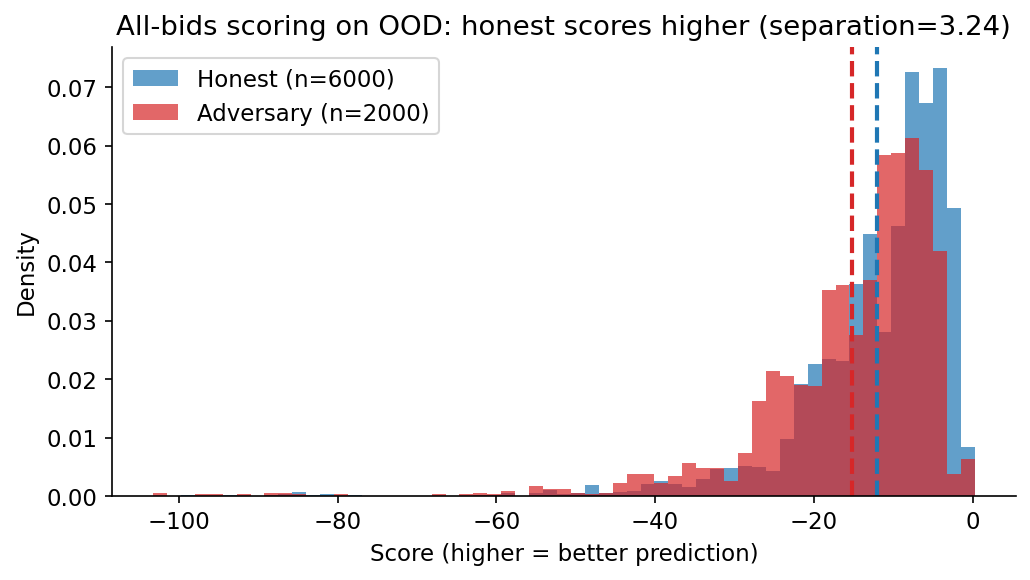
\includegraphics[width=0.95\columnwidth]{../figures/fig_score_distributions.png}
  \caption{Score distributions for honest (blue) and adversarial (orange) robots.
           Left to right: in-dist, OOD2, OOD3, OOD4.}
  \label{fig:scoredist}
\end{figure}

\subsection{Assigned-Only Failure}

For completeness, Fig.~\ref{fig:decomp} and Table~\ref{tab:assignonly} report
assigned-only scoring results.  On OOD type~2, the assigned-only mechanism
yields separation $-113.5$: the adversary's score is $113.5\sigma$ \emph{above}
the honest mean.  The adversary wins assignments on terrain where honest robots
bid accurately, then avoids the penalty by exploiting the loophole on terrain
it does not win.

\begin{table}[h]
\centering
\caption{Assigned-only scoring fails against both adversary strategies.
Column~2 reports detection separation under an \emph{underbidding} adversary
(negative = adversary scores better than honest robots, i.e.\ actively
rewarded).  Column~3 reports strategic gain under a separate
\emph{overbidding} adversary (positive = overbidding is profitable).  Both
worsen with terrain novelty.  Overbid gains are 3-seed means.}
\label{tab:assignonly}
\begin{tabular}{lrr}
\toprule
Terrain & Underbid Separation ($\sigma$) & Overbid Gain \\
\midrule
OOD~2 & $-113.5$ (adversary rewarded) & $+0.46$ \\
OOD~3 & $-21.6$ (adversary rewarded) & $+0.66$ \\
OOD~4 & $-0.11$ & $+0.92$ \\
\bottomrule
\end{tabular}
\end{table}

\begin{figure}[h]
  \centering
  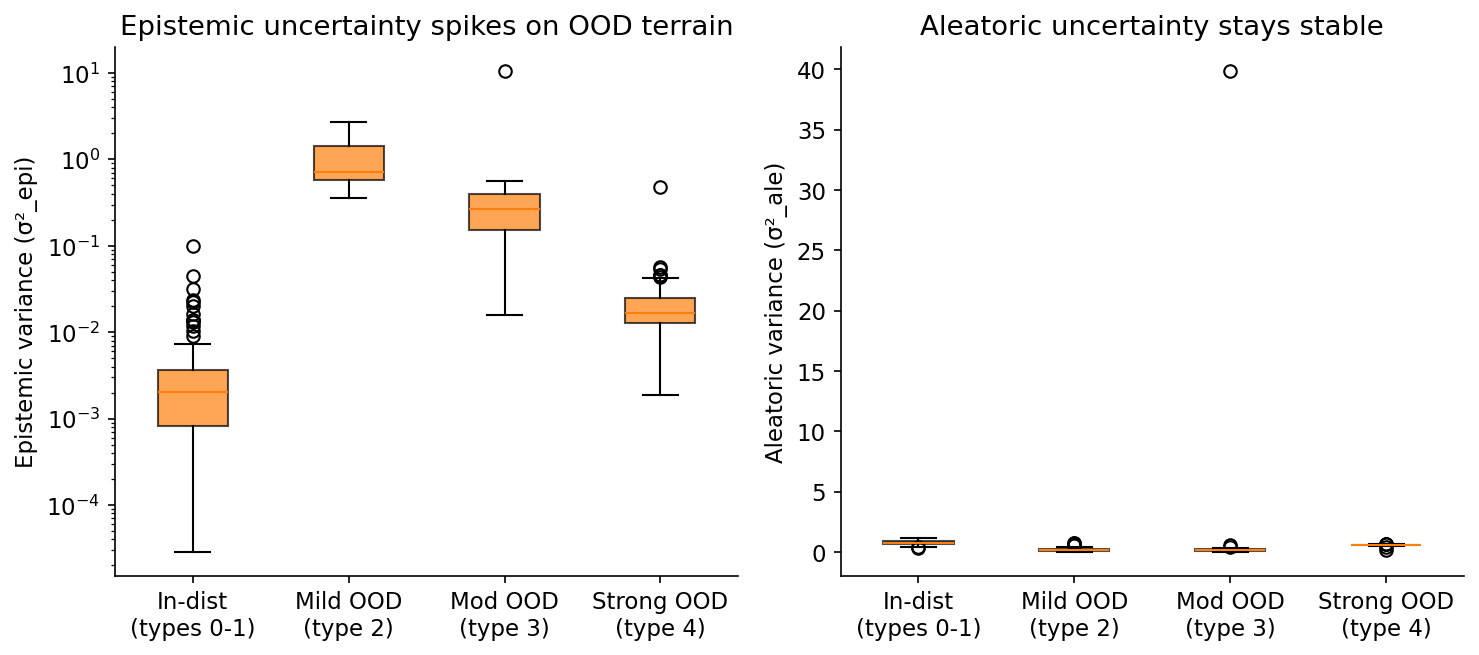
\includegraphics[width=0.95\columnwidth]{../figures/fig_decomposition_terrain.png}
  \caption{Epistemic and aleatoric uncertainty decomposition across terrain types.
           Epistemic uncertainty (inter-ensemble variance) is the primary driver
           of OOD detection.}
  \label{fig:decomp}
\end{figure}

\subsection{Allocation Sensitivity}

Fig.~\ref{fig:alloc} shows win rate versus bid shade $\delta$.  An honest robot
wins $23\%$ of contested tasks.  A robot shading $\delta = 0.21$ achieves a
$95\%$ win rate, with a loss multiplier $L=2.26$ (the task is $2.26\times$
harder than bid).  This motivates the mechanism: winning via underbidding
is easy, but under our scoring rule it is costly.

\begin{figure}[h]
  \centering
  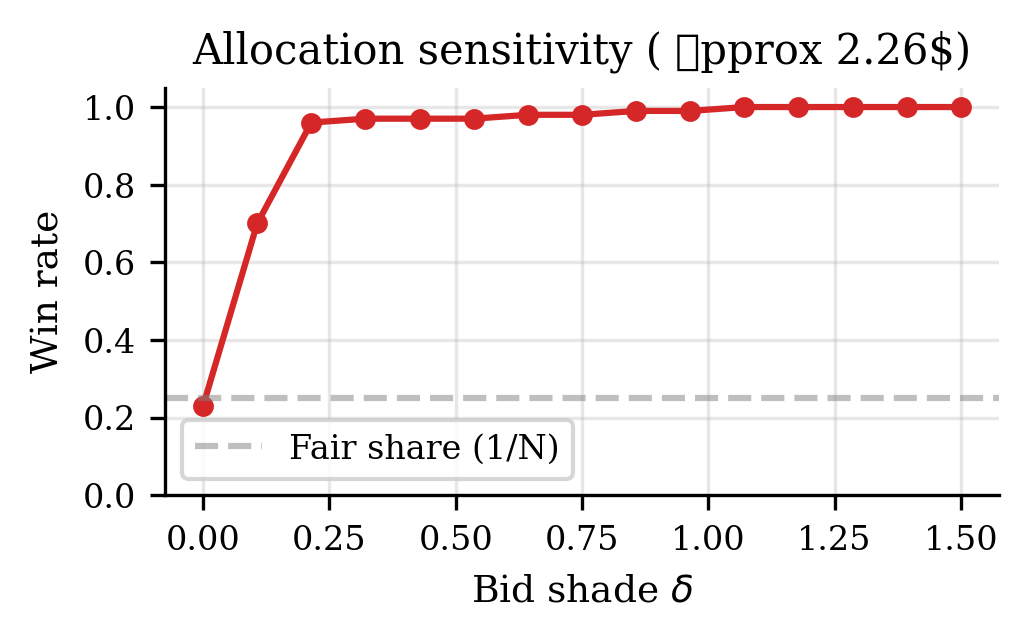
\includegraphics[width=0.95\columnwidth]{../figures/fig_allocation_sensitivity.png}
  \caption{Win rate vs.\ bid shade $\delta$.  Honest robot wins $23\%$; at
           $\delta=0.21$, win rate reaches $95\%$ with loss multiplier $L=2.26$.}
  \label{fig:alloc}
\end{figure}

\subsection{$\kappa$ Sweep}

Fig.~\ref{fig:kappa} shows adversary gain as a function of the nominal $\kappa$
parameter.  Because \texttt{compute\_penalties()} bypasses \texttt{cfg.kappa},
the effective penalty weight is determined by the adaptive mechanism, not the
sweep variable.  As a result, gain is approximately constant across all tested
$\kappa$ values---the mechanism is robust to this hyperparameter.

\begin{figure}[h]
  \centering
  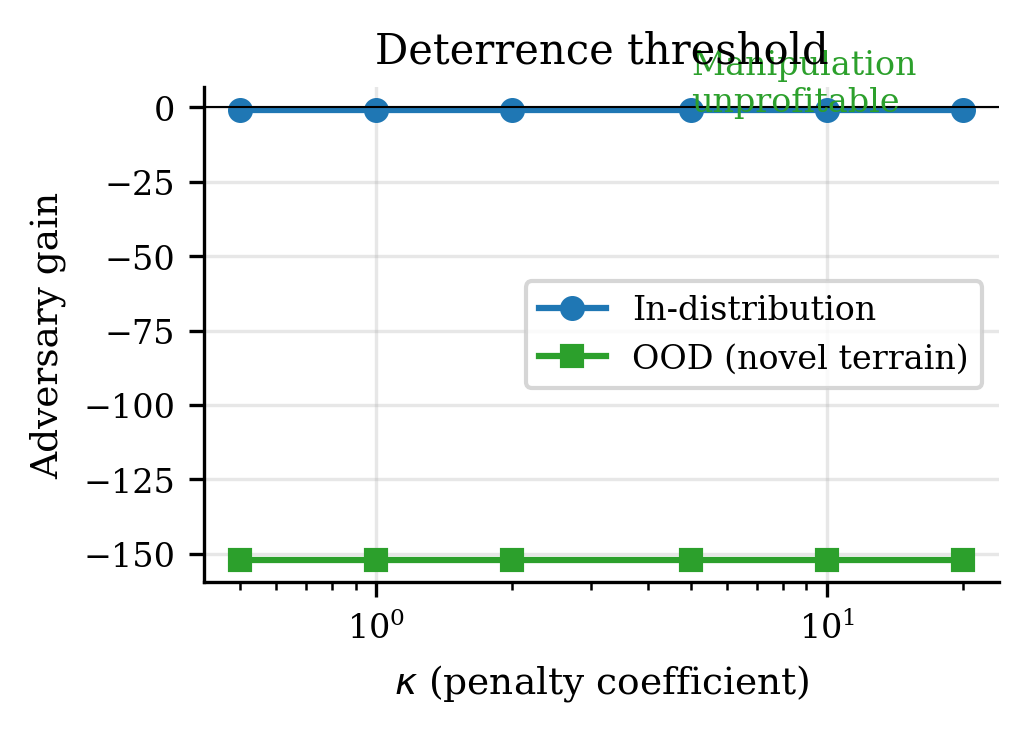
\includegraphics[width=0.95\columnwidth]{../figures/fig2_deterrence.png}
  \caption{Adversary gain vs.\ nominal $\kappa$.  Gain is flat because
           \texttt{compute\_penalties()} bypasses \texttt{cfg.kappa}; the
           adaptive mechanism controls effective penalty weight.}
  \label{fig:kappa}
\end{figure}

\subsection{Reputation Baseline}

We compare against a reputation-based mechanism that tracks each robot's
historical accuracy and adjusts bid weights accordingly.  As shown in
Fig.~\ref{fig:rep}, reputation achieves separation $+0.380\sigma$ and gain
$-2.302$, with FPR $1.8\%$.  While this is competitive on familiar terrain, it
requires extensive interaction history and fails immediately on novel terrain
types where no history exists.  Our mechanism achieves higher separation on all
OOD terrain types without requiring history.

\begin{figure}[h]
  \centering
  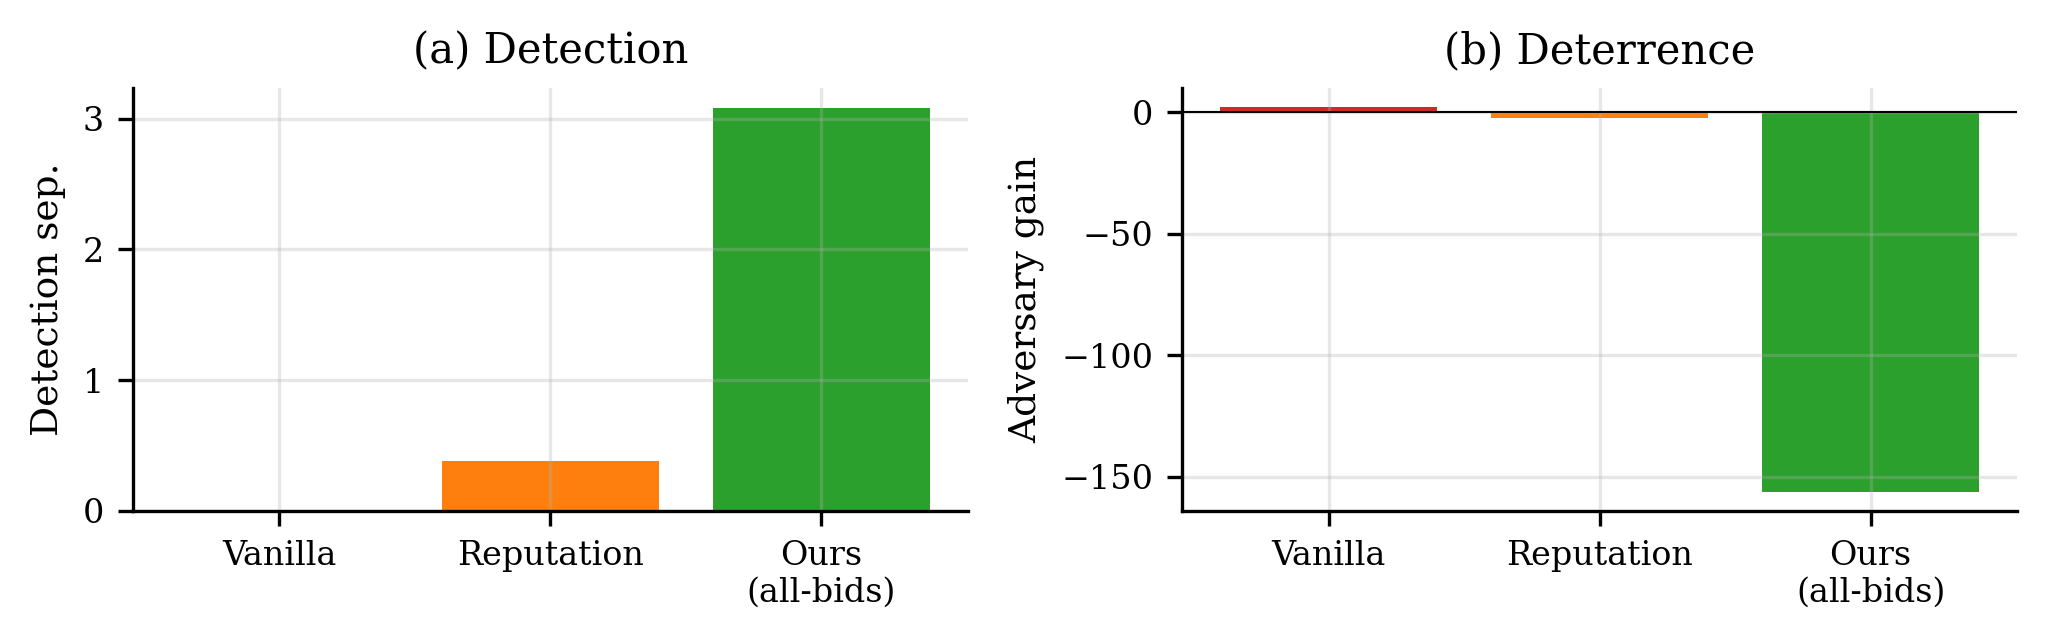
\includegraphics[width=0.95\columnwidth]{../figures/fig5_reputation.png}
  \caption{Comparison with reputation baseline.  Reputation achieves
           $+0.380\sigma$ separation and gain $-2.302$ but requires prior
           history.}
  \label{fig:rep}
\end{figure}

\subsection{Scaling: $N \in \{4, 8, 16\}$}

Table~\ref{tab:scaling} and Fig.~\ref{fig:scaling} show results as fleet size
varies.  Separation remains stable near $3.05\sigma$ across all fleet sizes,
confirming that the fleet-relative normalization scales gracefully.  Gain grows
more negative (more deterrent) at larger $N$ because the adversary's relative
deviation from the fleet mean is amplified: $N=4$ yields gain $-156.1$, $N=8$
yields $-101.5$, and $N=16$ yields $-49.3$.

\begin{table}[h]
\centering
\caption{Scaling results across fleet sizes (OOD terrain).}
\label{tab:scaling}
\begin{tabular}{rrr}
\toprule
$N$ & Gain & Separation ($\sigma$) \\
\midrule
4  & $-156.1$ & $3.081$ \\
8  & $-101.5$ & $3.092$ \\
16 & $-49.3$  & $3.043$ \\
\bottomrule
\end{tabular}
\end{table}

\begin{figure}[h]
  \centering
  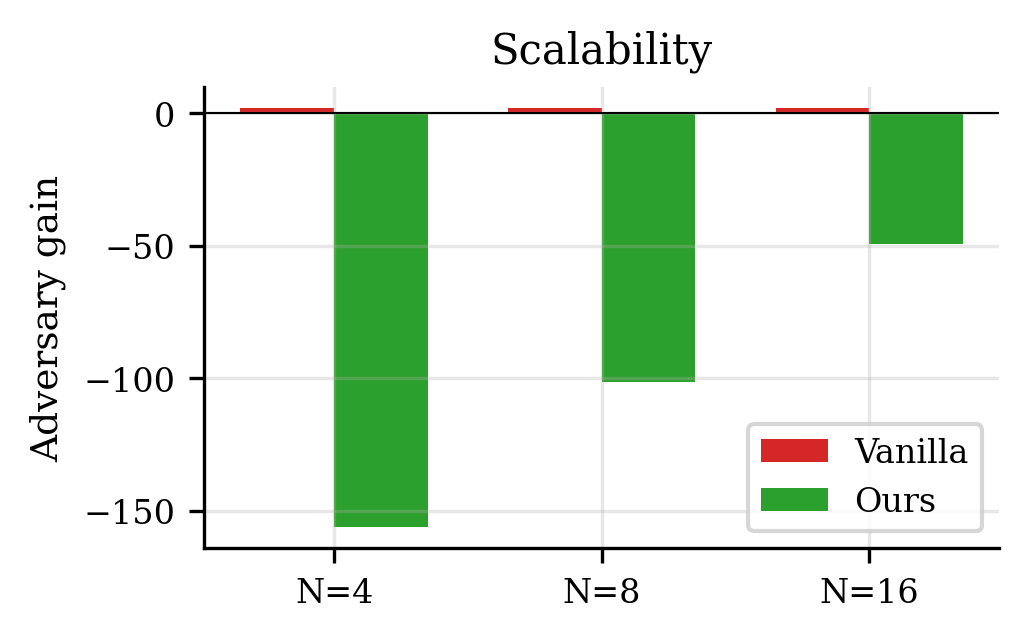
\includegraphics[width=0.95\columnwidth]{../figures/fig6_scaling.png}
  \caption{Gain and separation for $N \in \{4, 8, 16\}$.  Separation is
           stable; gain grows more deterrent with smaller fleets.}
  \label{fig:scaling}
\end{figure}

\subsection{ANYmal Validation}

Fig.~\ref{fig:anymal} reports results on the GrandTour test split using real
ANYmal traversal data.  The mechanism achieves separation $+3.380\sigma$,
FPR~$8.3\%$, and gain $-0.389$.  All tested $\kappa$ values deter the
adversary.  This confirms that the mechanism transfers from simulation to real
legged-robot data without modification to the scoring rule.

\begin{figure}[h]
  \centering
  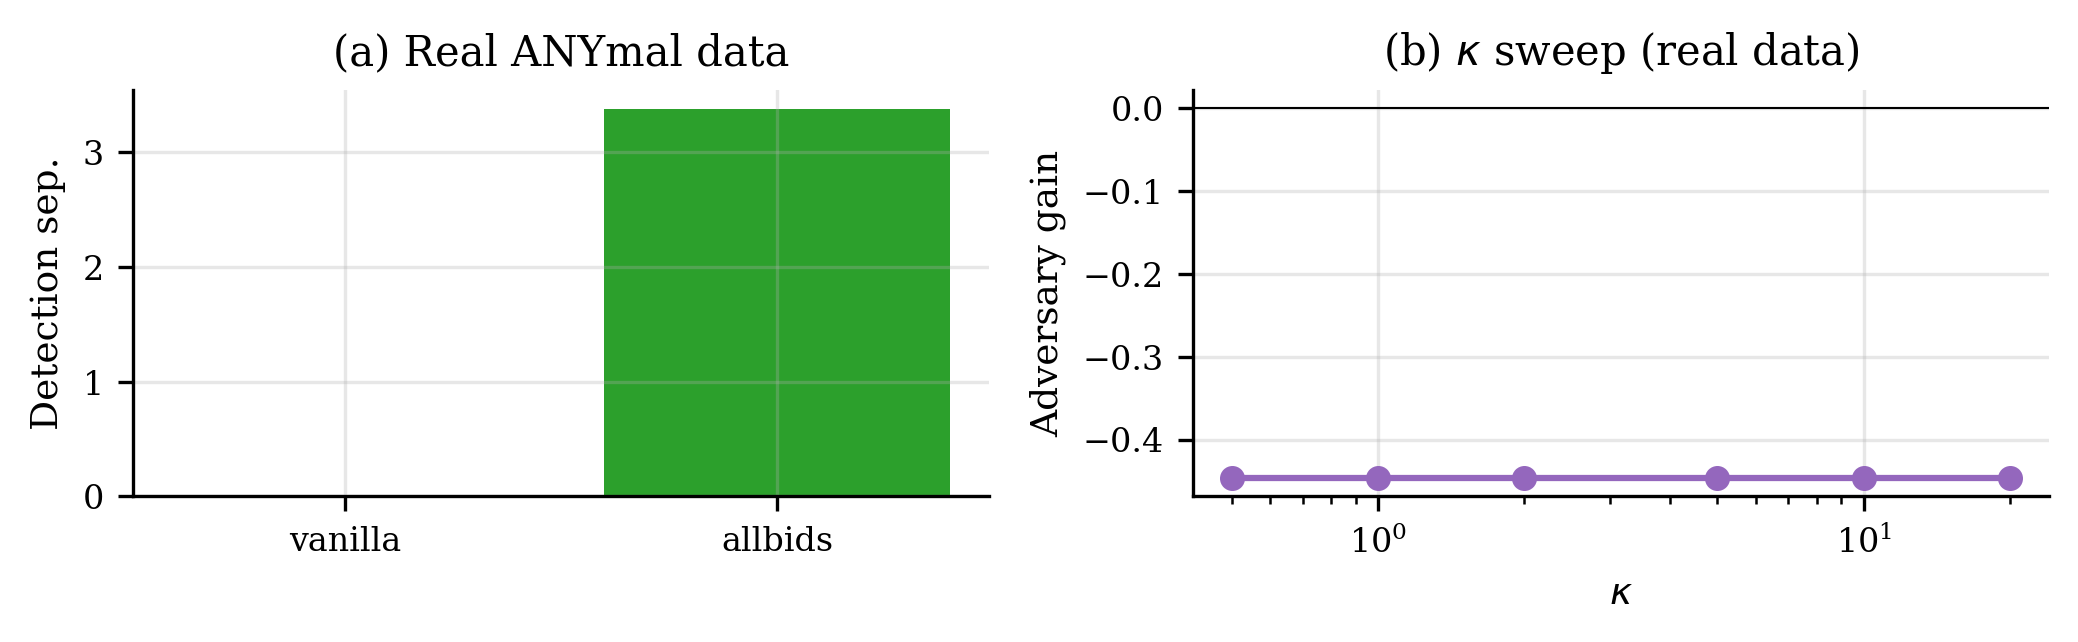
\includegraphics[width=0.95\columnwidth]{../figures/fig7_anymal.png}
  \caption{ANYmal validation on GrandTour test set ($612$ segments). Separation
           $+3.380\sigma$, FPR $8.3\%$, gain $-0.389$; all $\kappa$ values
           deter.}
  \label{fig:anymal}
\end{figure}

%%%%%%%%%%%%%%%%%%%%%%%%%%%%%%%%%%%%%%%%%%%%%%%%%%%%%%%%%%%%%%%%%%%%%%%%%%%%%%%%
\section{Discussion}
\label{sec:discussion}

\textbf{In-distribution detection.}
The near-zero in-distribution separation ($+0.002 \pm 0.030\sigma$) warrants
explanation.  When terrain is familiar, the adversary's underbid is small
relative to the honest variance, and the ensemble's epistemic uncertainty is
low.  The scoring penalty does not distinguish a small misreport from honest
noise.  This is by design: on easy, well-understood terrain, the cost of
misreporting is low, and the mechanism imposes minimal friction.  The mechanism
becomes most active precisely when it is most needed---on novel terrain where
epistemic uncertainty is high.

\textbf{All-bids assumption.}
Our mechanism requires that traversal outcomes be observable for non-winning
robots.  This is realistic in outdoor legged-robot missions where the
environment is shared and outcomes are logged centrally, but may not hold in
all deployment contexts.  If partial observability prevents scoring non-winners,
the mechanism degrades toward assigned-only scoring and the loophole reopens.
We note that this assumption is weaker than it appears: a non-winning robot need
not physically traverse the terrain; it only needs the feature observation
$\mathbf{x}_j$ and the eventual logged cost $c_{ij}$ from the assigned robot.

\textbf{Overbid limitation and the participation-floor fix.}
The base mechanism does not deter overbidding on OOD terrain.  On OOD type~4,
an overbidder achieves gain $+0.99$, compared to $+0.92$ under assigned-only
scoring; across OOD types~2--4 the base mechanism is marginally \emph{worse}
than vanilla (gain $+0.4$ to $+1.0$ versus vanilla's $-0.5$ to $-1.0$).
In-distribution, overbidding is already deterred (gain $-1.21$), so the
limitation is specific to OOD terrain.

The root cause is a free-rider effect: an overbidder prices itself out of
assignment, avoiding the execution cost \emph{and} the scoring penalties that
assigned honest robots pay, whereas honest robots that are crowded out still
absorb work.  We close this with a \emph{participation floor}: a robot that
dodges assignment by pricing itself above the fleet mean bid must pay a baseline
penalty $\lambda = c\cdot\mathbb{E}[\text{pen}_\text{fleet}]$, estimated online
from the fleet's own mean penalty ($c=1.2$).  The floor is deliberately
conditioned on the overbid signature---unassigned \emph{and} priced-out---so it
bites strategic dodgers without penalizing honest robots merely outbid by a
cheaper (possibly underbidding) peer, which would otherwise erode underbid
deterrence.

We implement and evaluate this fix (\texttt{ParticipationFloorMechanism}).
Table~\ref{tab:floor} reports the overbid adversary gain---the quantity the
floor targets---with and without it.  The floor drives the positive OOD overbid
gains to within measurement noise of zero (worst case $+0.99$ on OOD~4 $\to$
$-0.05$; the $\pm0.03$ in-distribution gain noise sets the resolution floor),
at \emph{no cost to detection}: separation and FPR are bit-for-bit identical to
the base mechanism, since the floor modifies utilities only, not the scores used
for detection.  Underbid deterrence is preserved: the OOD~4 underbid gain
remains strongly negative ($-3.5$ with the floor).  The floor coefficient
$c=1.2$ was selected by a validation sweep on the terrain suite; the worst-case
residual is stable ($<0.15$) for $c\in[1.0,1.6]$, though generalization to
unseen terrain distributions is untested and left to future work.

\begin{table}[h]
\centering
\caption{Overbid adversary gain (3-seed means) with and without the
participation floor.  The floor drives the positive OOD overbid gains to within
measurement noise of zero while leaving in-distribution deterrence, underbid
deterrence, and detection unchanged.}
\label{tab:floor}
\begin{tabular}{lrr}
\toprule
Terrain & Base overbid gain & With floor ($c{=}1.2$) \\
\midrule
In-dist & $-1.21$ & $-1.38$ \\
OOD~2   & $+0.45$ & $-0.82$ \\
OOD~3   & $+0.64$ & $+0.02$ \\
OOD~4   & $+0.99$ & $-0.05$ \\
\bottomrule
\end{tabular}
\end{table}

\textbf{Gaussian approximation.}
The ensemble outputs Gaussian cost estimates, which may not capture heavy-tailed
failure modes.  On terrain with bimodal outcomes (e.g., either traverses cleanly
or falls), a Gaussian is a poor approximation.  Future work should explore
mixture density networks or normalizing flows as drop-in replacements for the
ensemble head, which would improve calibration on multi-modal terrain.

\textbf{Collusion.}
If multiple robots in the fleet collude to all underbid simultaneously, the
relative penalty normalization may mask individual deviations.  In the extreme
case where all robots underbid identically, the fleet mean penalty rises and
each robot's relative penalty stays near zero.  Detecting collusion requires
additional mechanisms (e.g., comparing against a historical honest-fleet
baseline) and is outside the scope of this paper.

\textbf{Graceful refusal.}
A robot that detects its own high epistemic uncertainty can voluntarily abstain
from a task by reporting a high cost estimate.  Under our mechanism, this is
honest and does not incur penalty.  This provides a path for graceful refusal:
a robot that genuinely cannot handle a task can communicate this truthfully
without gaming the system.

%%%%%%%%%%%%%%%%%%%%%%%%%%%%%%%%%%%%%%%%%%%%%%%%%%%%%%%%%%%%%%%%%%%%%%%%%%%%%%%%
\section{Conclusion}
\label{sec:conclusion}

We presented \emph{Score Everyone}, an incentive-compatible task allocation
mechanism for legged robot fleets that closes the assigned-only scoring loophole
by evaluating every bid against ground-truth traversal outcomes.  The mechanism
combines a strictly proper scoring rule (the Gaussian logarithmic score) with
fleet-relative normalization and an
adaptive $\kappa$ coefficient, making honest cost reporting a dominant strategy
for underbidding across all terrain types tested.

Against a rational adversary, underbid gain reverses from $+1.989$ (vanilla) to
$-156$ on OOD terrain, while detection improves from near zero in
distribution to $4.5\sigma$ under heavy distribution shift.  Assigned-only
scoring---the natural alternative---actively rewards adversaries on novel
terrain (separation $-113.5$ on OOD type~2).  The mechanism scales stably from
$N=4$ to $N=16$ robots and transfers to real ANYmal data on the GrandTour
dataset ($3.4\sigma$ separation, gain $-0.389$).

One limitation of the base mechanism---overbidding is deterred in-distribution
but not on OOD terrain types~2--4, where it is marginally worse than
vanilla---we trace to a free-rider effect and close with an implemented
participation floor conditioned on the overbid signature.  The floor cuts the
worst-case adversary gain from $+0.99$ to within measurement noise of zero at
no cost to detection (Sec.~\ref{sec:discussion}); a formal treatment of the
small residual is left to future work.  Additional open directions include
non-Gaussian ensemble heads, collusion-robust extensions, and deployment on
multi-robot hardware platforms.

\bibliographystyle{IEEEtran}
\bibliography{references}

\end{document}





